\chapter{Remarks on the Method of Statistical Analysis}\label{appendix:analysis-remarks}
Many studies utilizing the \ac{5D-ASC} scoring or the \ac{11-ASC} scoring (such as \textcites{carbonaro2018double}{holze2020distinct}{holze2021acute}{hutten2020mood}) use statistical tests which require normally distributed variables (repeated-measures analysis of variance, paired t-test), to compare the resulting questionnaire scores of placebo and non-placebo groups. Our study has used the same approach, but we identified an issue with this approach, which may be relevant to the field.

The issue stems from the fact that the \acf{VAS}, which is the method participants answer to the questions of the questionnaire, results in bounded measurements in the interval $[0\%; 100\%]$. After applying this questionnaire in our study, we found out, that for the control scenario, many of the questions were answered with $0\%$, as can also be seen in the aforementioned studies. This results in the mean of the resulting factors, which are also bounded by the same interval as the answers themselves, being very close to the lower bound of $0\%$.

It may be a mistake to assume that the resulting factors are normally distributed, if, for example, their 95\% confidence interval (of the assumed normal distribution) reaches outside of the $[0\%; 100\%]$ bounds. This can also be seen in figures \ref{fig:results-5d-asc} and \ref{fig:results-11-asc}. It seems that some studies prefer to mask this issue by visualising the error of the resulting factors using the standard error (SE), which is essentially a 68\% confidence interval. However, the preferred measure for precision in medicine is the 95\% confidence interval \autocite{lang2004twenty}, so the usage of the SE may be misleading. When interpreting data with the SE, it helps to remember that the 95\% confidence interval of a normal distribution is roughly twice (\tildec1.96) as large as the 68\% interval denoted by the SE.

As an alternative, it may be much more appropriate to use a bounded distribution to model the resulting factors instead. The following two may be suitable:

\begin{enumerate}
    \item The logit-normal distribution: If $X$ is logit-normally distributed, then $Y = \operatorname{logit}(X) = \ln(\frac{X}{1 - X})$ is normally distributed. Essentially, the $\operatorname{logit}$ transform stretches the lower (0) and upper (1) bounds to infinity (see figure \ref{fig:graph-logit}). However, the $\operatorname{logit}$ transform's domain is an open interval $(0; 1)$, rather than a closed interval $[0; 1]$, which prevents it from being usable with measurements at the bounds. This is, unfortunately, the case for the psychometric questionnaire used in this study, as participants may answer with $0\%$ or $100\%$.
    \item The beta distribution: Doesn't suffer from the necessity of using a transform that would be undefined at the bounds. Possibly even more expressive than the logit-normal distribution.
\end{enumerate}

I suspect the main challenge of using these alternative distributions comes with the testing of hypotheses. With these distributions, we can no longer use standard statistical methods of analysis only applicable to normally distributed data.

I don't believe this finding invalidates past studies, but it may serve as a place for improvement of future ones.

% PDFs
\def\pdfnorm(#1, #2, #3){((1 / ((#3) * sqrt(2 * pi))) * exp(-0.5 * ((#1) - (#2))^2 / ((#3)^2)))}

% gnuplot only
\def\B(#1, #2){((gamma(#1) * gamma(#2)) / gamma((#1) + (#2)))}
\def\pdfbeta(#1, #2, #3){((((#1)^((#2) - 1)) * ((1 - (#1))^((#3) - 1))) / \B(#2, #3))}

\def\logit(#1){(ln((#1)/(1-(#1))))}
\def\pdflogitnorm(#1, #2, #3){(\pdfnorm((\logit(#1)), (#2), (#3)) / ((#1) * (1 - (#1))))}

\begin{figure}[h]
    \centering

    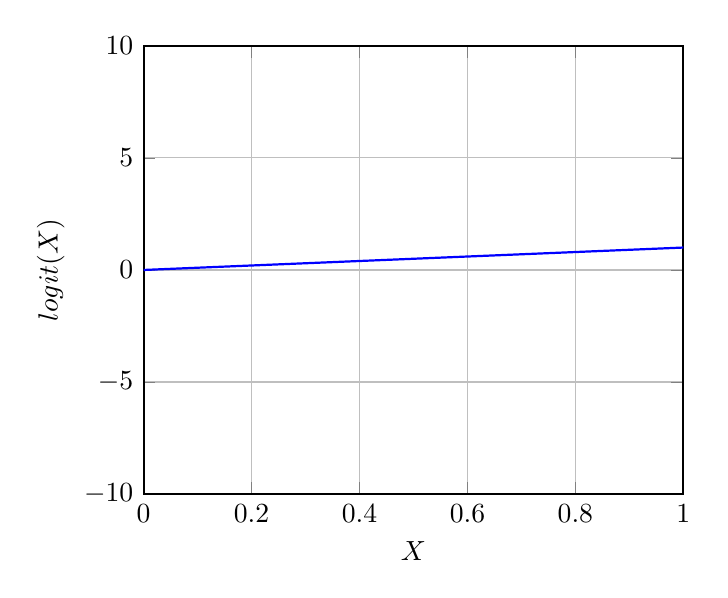
\begin{tikzpicture}
    \begin{axis}[
        xlabel={$X$},
        ylabel={$\operatorname{logit}(X)$},
        samples=1000,
        grid,
        thick,
        domain=0.0000001:0.9999999,
        xmin=0,
        xmax=1,
        ymin=-10,
        ymax=10,
        legend pos=outer north east,
    ]

        \addplot+ [no marks] { \logit(x) };

    % \addlegendentry{y=$\operatorname{logit}(x)$}
    \end{axis}
    \end{tikzpicture}

    \caption{
        The $\operatorname{logit}$ transform.
    }
    \label{fig:graph-logit}
\end{figure}

\begin{figure}[h]
    \centering
    \subfloat[\centering Examples of logit-normal distributions of random variable $X$.]{
        \begin{tikzpicture}
        \begin{axis}[
            width=6cm,
            xlabel={$x$},
            ylabel={$f_{\operatorname{logit-normal}}(x)$},
            samples=200,
            grid,
            thick,
            domain=0.0000001:0.9999999,
            xmin=0,
            xmax=1,
            ymin=0,
            ymax=10,
            legend pos=outer north east,
            cycle list name=exotic,
        ]

            \addplot+ [no marks] { \pdflogitnorm(x, 0, 1) };
            \addplot+ [no marks] { \pdflogitnorm(x, 1, 1) };
            \addplot+ [no marks] { \pdflogitnorm(x, -1, 2) };
            \addplot+ [no marks] { \pdflogitnorm(x, 2, 0.5) };

        % \addlegendentry{y=$\operatorname{logit}(x)$}
        \end{axis}
        \end{tikzpicture}
    }%
    \quad
    \subfloat[\centering The corresponding normal distributions of $Y = \operatorname{logit}(X)$.]{
        \begin{tikzpicture}
        \begin{axis}[
            width=6cm,
            xlabel={$x$},
            ylabel={$f_{\operatorname{normal}}(x)$},
            samples=200,
            grid,
            thick,
            domain=-5:5,
            xmin=-5,
            xmax=5,
            ymin=0,
            ymax=1,
            legend pos=outer north east,
            cycle list name=exotic,
        ]

            \addplot+ [no marks] { \pdfnorm(x, 0, 1) };
            \addplot+ [no marks] { \pdfnorm(x, 1, 1) };
            \addplot+ [no marks] { \pdfnorm(x, -1, 2) };
            \addplot+ [no marks] { \pdfnorm(x, 2, 0.5) };

        % \addlegendentry{y=$\operatorname{logit}(x)$}
        \end{axis}
        \end{tikzpicture}
    }%
    \caption{Examples of the logit-normal distribution and their corresponding normal distributions.}%
    \label{fig:mordvintsev2015inceptionism}%
\end{figure}

\begin{figure}[h]
    \centering

    \begin{tikzpicture}
    \begin{axis}[
        xlabel={$x$},
        ylabel={$f_{\operatorname{beta}}$},
        samples=200,
        grid,
        thick,
        domain=0.0000001:0.9999999,
        xmin=0,
        xmax=1,
        ymin=0,
        ymax=10,
        cycle list name=exotic,
        % restrict y to domain,
        % legend pos=outer north east,
    ]

        \addplot+ [no marks] gnuplot { \pdfbeta(x, 2, 2) };
        \addplot+ [no marks] gnuplot { \pdfbeta(x, 2, 5) };
        \addplot+ [no marks] gnuplot { \pdfbeta(x, 1, 5) };
        \addplot+ [no marks] gnuplot { \pdfbeta(x, 50, 10) };
        \addplot+ [no marks] gnuplot { \pdfbeta(x, 1, 1) };

    % \addlegendentry{y=$\operatorname{logit}(x)$}
    \end{axis}
    \end{tikzpicture}

    \caption{
        Examples of the beta distribution. Note that the beta distribution, as opposed to the logit-normal distribution, is also able to express a uniform distribution with parameters $\alpha=1, \beta=1$.
    }
    \label{fig:graph-pdf-beta}
\end{figure}
